\chapter{Mathematical Derivations}
\label{app:deriv}

This appendix collects, in self-contained form, the analytical machinery underlying the plasma-sheath model and the inversion framework used throughout the monograph. It proceeds from first principles: the Poisson--Boltzmann equation is linearised to recover the electron Debye length; the cold-ion fluid sheath equation is expanded to obtain the Bohm criterion; the collisionless, space-charge-limited sheath is solved to yield the Child--Langmuir law and its matrix-sheath limit; a kinetic flux-balance argument produces the floating-potential expression; the ion energy flux is defined as a velocity-space moment of the ion distribution function; and the Tikhonov-regularised least-squares estimator and its Bayesian MAP counterpart are derived for reconstructing the ion energy flux from noisy diagnostic data. $T_{\mathrm{e}}$ and $T_{\mathrm{i}}$ denote electron and ion temperatures multiplied by Boltzmann's constant $k_{\mathrm{B}}$, in energy units, so no explicit $k_{\mathrm{B}}$ appears below. Table~\ref{tab:notation} summarises the notation used.

\begin{table}[htbp]
\centering
\caption{Summary of the principal symbols used in this appendix. All temperatures are expressed in energy units, following the convention $T_{\mathrm{e}} \equiv k_{\mathrm{B}} T_{\mathrm{e,phys}}$.}
\label{tab:notation}
\begin{tabular}{@{}ll@{}}
\toprule
Symbol & Meaning \\
\midrule
$n_{\mathrm{e}}, n_{\mathrm{i}}$ & Electron and ion number densities \\
$T_{\mathrm{e}}, T_{\mathrm{i}}$ & Electron and ion temperatures (energy units) \\
$\lambda_{\mathrm{D}}$ & Electron Debye length \\
$u_{\mathrm{B}}$ & Bohm velocity \\
$\phi(x)$ & Electrostatic potential, referenced to the bulk plasma \\
$V_{\mathrm{f}}$ & Floating potential \\
$f_{\mathrm{i}}(v)$ & Ion velocity distribution function \\
$\Gamma_{\mathrm{i}}$ & Ion particle flux density \\
$\Gamma_{E}$ & Ion energy flux density \\
$m_{\mathrm{i}}, m_{\mathrm{e}}$ & Ion and electron mass \\
$e, \varepsilon_{0}$ & Elementary charge, vacuum permittivity \\
$\mathbf{K}, \mathbf{L}$ & Forward (kernel) and regularisation operators \\
$\alpha$ & Tikhonov regularisation parameter \\
$\boldsymbol{\Sigma}_{d}, \boldsymbol{\Sigma}_{m}$ & Data and prior (model) covariance matrices \\
\bottomrule
\end{tabular}
\end{table}

\section{The Debye Length from the Poisson--Boltzmann Equation}
\label{appA-sec:debye}

\subsection{Statement of the problem}

Consider a quasi-neutral plasma of unperturbed density $n_{0}$ with singly charged ions and Maxwellian electrons at temperature $T_{\mathrm{e}}$. A small local perturbation of the potential $\phi(\mathbf{r})$ -- near a probe, a wall, or a test charge -- disturbs the electron density via the Boltzmann relation, while the massive ions act, to leading order, as an immobile neutralising background, as in the plasma-wall transition problem linking the quasi-neutral bulk to the space-charge sheath \cite{ref0013}. The goal is the characteristic screening length of such a perturbation.

\subsection{Poisson's equation}

The electrostatic potential obeys Poisson's equation,
\begin{equation}
\nabla^{2}\phi(\mathbf{r}) = -\frac{\rho(\mathbf{r})}{\varepsilon_{0}} = -\frac{e\big[n_{\mathrm{i}}(\mathbf{r}) - n_{\mathrm{e}}(\mathbf{r})\big]}{\varepsilon_{0}},
\label{eq:poisson0}
\end{equation}
with $\rho$ the local net charge density and $e$ the elementary charge. In one-dimensional planar geometry, sufficient here, this becomes
\begin{equation}
\frac{\mathrm{d}^{2}\phi}{\mathrm{d}x^{2}} = -\frac{e\big[n_{\mathrm{i}}(x) - n_{\mathrm{e}}(x)\big]}{\varepsilon_{0}}.
\label{eq:poisson1d}
\end{equation}

\subsection{The Boltzmann relation and linearisation}

Electrons remain close to thermal equilibrium in a slowly varying potential, so their density follows the Boltzmann relation,
\begin{equation}
n_{\mathrm{e}}(x) = n_{0}\exp\!\left[\frac{e\phi(x)}{T_{\mathrm{e}}}\right],
\label{appA-eq:boltzmann}
\end{equation}
with $\phi \to 0$, $n_{\mathrm{e}} \to n_{0}$ far from the perturbation \cite{ref0013,ref0670}. Taking the ions as a rigid background, $n_{\mathrm{i}}(x) = n_{0}$, substitution into Eq.~\eqref{eq:poisson1d} yields the nonlinear Poisson--Boltzmann equation,
\begin{equation}
\frac{\mathrm{d}^{2}\phi}{\mathrm{d}x^{2}} = \frac{e n_{0}}{\varepsilon_{0}}\left(\exp\!\left[\frac{e\phi}{T_{\mathrm{e}}}\right] - 1\right).
\label{eq:pb_nonlinear}
\end{equation}
For a weak perturbation, $|e\phi/T_{\mathrm{e}}| \ll 1$, linearising the exponential, $\exp(e\phi/T_{\mathrm{e}}) \approx 1 + e\phi/T_{\mathrm{e}}$, gives the linear screening equation
\begin{equation}
\frac{\mathrm{d}^{2}\phi}{\mathrm{d}x^{2}} = \frac{n_{0}e^{2}}{\varepsilon_{0}T_{\mathrm{e}}}\,\phi \equiv \frac{\phi}{\lambda_{\mathrm{D}}^{2}},
\label{eq:linearised}
\end{equation}
which defines the electron Debye length
\begin{equation}
\boxed{\lambda_{\mathrm{D}} \equiv \sqrt{\frac{\varepsilon_{0}T_{\mathrm{e}}}{n_{0}e^{2}}}}.
\label{appA-eq:debye}
\end{equation}

\subsection{Solution and physical interpretation}

The general solution of Eq.~\eqref{eq:linearised} is $\phi(x) = A\,e^{x/\lambda_{\mathrm{D}}} + B\,e^{-x/\lambda_{\mathrm{D}}}$. Requiring $\phi \to 0$ as $x \to +\infty$ forces $A=0$; matching $\phi(0) = \phi_{0}$ gives
\begin{equation}
\phi(x) = \phi_{0}\exp\!\left(-\frac{x}{\lambda_{\mathrm{D}}}\right).
\label{eq:debye_profile}
\end{equation}
Thus $\lambda_{\mathrm{D}}$ is the $e$-folding screening length separating the quasi-neutral bulk from the non-neutral sheath (Sections~\ref{appA-sec:bohm}, \ref{sec:cl}). For $n_{0} = \SI{1e16}{\per\cubic\meter}$, $T_{\mathrm{e}} = \SI{3}{\electronvolt}$, Eq.~\eqref{appA-eq:debye} gives $\lambda_{\mathrm{D}} \approx \SI{1.29e-4}{\meter}$ ($\approx\SI{130}{\micro\meter}$), orders of magnitude below a typical vessel dimension, justifying the thin-sheath approximation.

Retaining ion mobility gives an analogous ion Boltzmann relation, $n_{\mathrm{i}}(x) = n_{0}\exp[-e\phi(x)/T_{\mathrm{i}}]$, linearising to an ion Debye length $\lambda_{\mathrm{Di}} = \sqrt{\varepsilon_{0}T_{\mathrm{i}}/(n_{0}e^{2})}$; the two combine in quadrature,
\begin{equation}
\frac{1}{\lambda_{\mathrm{D}}^{2}} = \frac{1}{\lambda_{\mathrm{De}}^{2}} + \frac{1}{\lambda_{\mathrm{Di}}^{2}},
\label{eq:combined_debye}
\end{equation}
with $\lambda_{\mathrm{De}}$ the electron Debye length of Eq.~\eqref{appA-eq:debye}. Since $T_{\mathrm{e}} \gtrsim T_{\mathrm{i}}$ in most low-temperature plasmas, $\lambda_{\mathrm{D}} \approx \lambda_{\mathrm{De}}$ is used elsewhere. Inside the sheath itself ions are supersonic and no longer respond adiabatically, so Eq.~\eqref{eq:combined_debye} applies only in the quasi-neutral bulk and presheath.

\subsection{Physical significance: the plasma parameter}

The derivation is self-consistent only if many electrons participate collectively in screening a single test charge, quantified by the plasma parameter -- the number of electrons within a sphere of radius $\lambda_{\mathrm{D}}$,
\begin{equation}
N_{\mathrm{D}} \equiv \frac{4}{3}\pi\lambda_{\mathrm{D}}^{3}n_{0}.
\label{eq:plasma_parameter}
\end{equation}
$N_{\mathrm{D}} \gg 1$ -- equivalently, mean electrostatic potential energy small compared with mean kinetic energy $T_{\mathrm{e}}$ -- marks a weakly coupled plasma dominated by collective Debye-screened behaviour, as opposed to a strongly coupled fluid where mean-field theory fails. For the parameters above, $N_{\mathrm{D}} \approx 9.0\times10^{4}$, confirming Eq.~\eqref{eq:pb_nonlinear} is fully justified \cite{ref0013}. This separation -- $\lambda_{\mathrm{D}}$ microscopic relative to device dimensions yet macroscopic relative to the interparticle spacing $n_{0}^{-1/3}$ -- lets the sheath be treated as a thin, quasi-1D boundary layer throughout.

\section{The Bohm Criterion from the Sheath Equation}
\label{appA-sec:bohm}

\subsection{Fluid description of the ion flow}

The Bohm criterion is the condition on ion drift velocity entering a sheath that guarantees a monotonic, non-oscillatory space-charge solution of Poisson's equation. First given by Bohm and refined since \cite{ref0001,ref0004,ref0015}, it is reproduced here for a cold, collisionless ion fluid entering the sheath along $x$ with density $n_{\mathrm{i}}(x)$ and drift speed $u_{\mathrm{i}}(x)$.

Steady-state continuity requires constant particle flux,
\begin{equation}
n_{\mathrm{i}}(x)\,u_{\mathrm{i}}(x) = n_{0}u_{0} \equiv \Gamma_{\mathrm{i}},
\label{eq:ion_cont}
\end{equation}
with $n_{0}$, $u_{0}$ the ion density and speed at the sheath edge $x=0$, $\phi(0)=0$. Neglecting collisions and pressure, the ion momentum equation integrates to
\begin{equation}
\tfrac{1}{2}m_{\mathrm{i}}u_{\mathrm{i}}^{2}(x) + e\phi(x) = \tfrac{1}{2}m_{\mathrm{i}}u_{0}^{2},
\label{eq:ion_energy}
\end{equation}
so
\begin{equation}
u_{\mathrm{i}}(x) = \left(u_{0}^{2} - \frac{2e\phi(x)}{m_{\mathrm{i}}}\right)^{1/2}.
\label{eq:ui_of_phi}
\end{equation}
Combining Eqs.~\eqref{eq:ion_cont} and~\eqref{eq:ui_of_phi} gives the ion density as a functional of $\phi$,
\begin{equation}
n_{\mathrm{i}}(\phi) = n_{0}\left(1 - \frac{2e\phi}{m_{\mathrm{i}}u_{0}^{2}}\right)^{-1/2}.
\label{eq:ni_of_phi}
\end{equation}
Electrons retain the Boltzmann relation, Eq.~\eqref{appA-eq:boltzmann}, so $n_{\mathrm{e}}(\phi) = n_{0}\exp(e\phi/T_{\mathrm{e}})$.

\subsection{Expansion about the sheath edge}

Substituting $n_{\mathrm{i}}(\phi)$, $n_{\mathrm{e}}(\phi)$ into Poisson's equation gives the sheath equation
\begin{equation}
\frac{\mathrm{d}^{2}\phi}{\mathrm{d}x^{2}} = \frac{en_{0}}{\varepsilon_{0}}\left[\exp\!\left(\frac{e\phi}{T_{\mathrm{e}}}\right) - \left(1 - \frac{2e\phi}{m_{\mathrm{i}}u_{0}^{2}}\right)^{-1/2}\right].
\label{eq:sheath_eq}
\end{equation}
Whether the sheath edge admits a monotonic rather than oscillatory potential has drawn extensive fluid and kinetic study \cite{ref0665,ref0666}. To extract the marginal condition, expand to first order in $e\phi$ as $\phi \to 0^{-}$:
\begin{align}
\exp\!\left(\frac{e\phi}{T_{\mathrm{e}}}\right) &\approx 1 + \frac{e\phi}{T_{\mathrm{e}}} + \mathcal{O}(\phi^{2}), \\
\left(1 - \frac{2e\phi}{m_{\mathrm{i}}u_{0}^{2}}\right)^{-1/2} &\approx 1 + \frac{e\phi}{m_{\mathrm{i}}u_{0}^{2}} + \mathcal{O}(\phi^{2}).
\end{align}
Subtracting, the zeroth-order terms cancel by quasi-neutrality, leaving
\begin{equation}
\frac{\mathrm{d}^{2}\phi}{\mathrm{d}x^{2}} \approx \frac{n_{0}e^{2}}{\varepsilon_{0}}\left(\frac{1}{T_{\mathrm{e}}} - \frac{1}{m_{\mathrm{i}}u_{0}^{2}}\right)\phi.
\label{eq:linearized_sheath}
\end{equation}

\subsection{The Bohm inequality}

Equation~\eqref{eq:linearized_sheath} has the form of Eq.~\eqref{eq:linearised}, with a coefficient whose sign depends on $u_{0}$: if positive, the perturbation decays back into the quasi-neutral plasma and no sheath forms; if negative, it admits growing, non-oscillatory solutions for $\phi<0$, consistent with a sheath falling monotonically toward a negatively biased wall. The marginal condition is therefore
\begin{equation}
\frac{1}{T_{\mathrm{e}}} - \frac{1}{m_{\mathrm{i}}u_{0}^{2}} \le 0
\quad\Longleftrightarrow\quad
m_{\mathrm{i}}u_{0}^{2} \ge T_{\mathrm{e}},
\end{equation}
i.e.
\begin{equation}
\boxed{u_{0} \ge u_{\mathrm{B}} \equiv \sqrt{\frac{T_{\mathrm{e}}}{m_{\mathrm{i}}}}},
\label{appA-eq:bohm}
\end{equation}
the Bohm criterion, $u_{\mathrm{B}}$ the Bohm velocity. Ions must enter the sheath supersonically with respect to $u_{\mathrm{B}}$; the quasi-neutral presheath satisfies this self-consistently, accelerating ions from rest through a potential drop of order $T_{\mathrm{e}}/(2e)$. How the marginal speed is attained at the sheath edge remains active \cite{ref0004}, including magnetised presheath structure \cite{ref0017}.

For argon at $T_{\mathrm{e}} = \SI{3}{\electronvolt}$, $m_{\mathrm{i}} = \SI{6.63e-26}{\kilo\gram}$, Eq.~\eqref{appA-eq:bohm} gives $u_{\mathrm{B}} \approx \SI{2.69e3}{\meter\per\second}$, recurring in Section~\ref{sec:cl}.

\subsection{Kinetic generalisation}

The fluid derivation assumes a cold, mono-energetic ion beam. The kinetic statement retains an arbitrary ion velocity distribution $f_{\mathrm{i}}(v)$ at the sheath edge, normalised so $n_{0} = \int_{0}^{\infty} f_{\mathrm{i}}(v)\,\mathrm{d}v$. Repeating the linearisation of Eq.~\eqref{eq:sheath_eq} for a distribution of speeds yields the kinetic Bohm criterion,
\begin{equation}
\int_{0}^{\infty} \frac{f_{\mathrm{i}}(v)}{v^{2}}\,\mathrm{d}v \le \frac{n_{0}m_{\mathrm{i}}}{T_{\mathrm{e}}},
\label{eq:kinetic_bohm}
\end{equation}
first placed on rigorous footing by Riemann \cite{ref0001} and extended since \cite{ref0004,ref0015}. It reduces to the fluid form, Eq.~\eqref{appA-eq:bohm}, in the cold-beam limit $f_{\mathrm{i}}(v) = n_{0}\delta(v-u_{0})$, and emphasises the disproportionate weight of \emph{slow} ions, since the integrand diverges as $v \to 0$ whenever the distribution has non-vanishing low-speed weight. The Tonks--Langmuir model, in which ions are born at rest throughout the presheath and accelerated collisionlessly, is the cleanest setting where Eq.~\eqref{eq:kinetic_bohm} holds as an equality at the sheath edge \cite{ref0665,ref0666}, fixing the sheath-edge location in kinetically self-consistent treatments.

\subsection{Magnetised and oblique-field generalisation}

Equation~\eqref{appA-eq:bohm} assumes one-dimensional, unconstrained ion flow. When a magnetic field $\mathbf{B}$ threads the sheath obliquely, ion motion perpendicular to $\mathbf{B}$ is constrained on the cyclotron time scale, and only the wall-normal drift component can satisfy the flux and energy-conservation arguments above. Repeating the sheath-edge expansion with velocity decomposed parallel/perpendicular to $\mathbf{B}$ shows a monotonic sheath now requires only the wall-normal component to exceed the Bohm speed,
\begin{equation}
u_{0,\perp\text{-wall}} \ge u_{\mathrm{B}} = \sqrt{\frac{T_{\mathrm{e}}}{m_{\mathrm{i}}}},
\label{eq:bohm_chodura}
\end{equation}
the Bohm--Chodura criterion. Because the field cannot accelerate ions along the wall normal, satisfying Eq.~\eqref{eq:bohm_chodura} generally requires an additional Chodura (magnetic presheath) layer, of thickness set by the ion Larmor radius rather than $\lambda_{\mathrm{D}}$, interposed between the bulk presheath and the electrostatic Debye sheath, analysed for oblique fields and kinetic trajectories \cite{ref0017}.

\section{The Child--Langmuir Law for a Matrix / Space-Charge Sheath}
\label{sec:cl}

\subsection{The collisionless, high-voltage sheath}

Once the ion flow satisfies the Bohm criterion, the sheath may, for sufficiently large wall bias, be treated as electron-free and space-charge-limited: $n_{\mathrm{e}} \ll n_{\mathrm{i}}$ everywhere except a thin transition layer, since the electron density falls off rapidly with the large negative potential via Eq.~\eqref{appA-eq:boltzmann}. This is the classical Child--Langmuir regime, examined within two-fluid presheath--sheath models \cite{ref0023}. We reproduce the derivation for a planar sheath of thickness $s$, sheath edge at $x=0$, $\phi=0$, wall at $x=s$ biased at $\phi(s) = -V_{0}$, $V_{0}>0$.

\subsection{Derivation}

Work with $V(x) \equiv -\phi(x)$, increasing monotonically from $V(0)=0$ to $V(s)=V_{0}$. Poisson's equation, with $n_{\mathrm{e}}\approx 0$, reads
\begin{equation}
\frac{\mathrm{d}^{2}V}{\mathrm{d}x^{2}} = \frac{e\,n_{\mathrm{i}}(x)}{\varepsilon_{0}}.
\label{eq:poisson_cl}
\end{equation}
Ion current continuity fixes a constant current density,
\begin{equation}
J = e\,n_{\mathrm{i}}(x)\,u_{\mathrm{i}}(x),
\label{eq:cl_cont}
\end{equation}
and, taking ions to enter with negligible kinetic energy compared with that gained falling through $V(x)$ (accurate as $eV_{0}/T_{\mathrm{e}} \to \infty$), energy conservation gives
\begin{equation}
\tfrac{1}{2}m_{\mathrm{i}}u_{\mathrm{i}}^{2}(x) = eV(x)
\quad\Longrightarrow\quad
u_{\mathrm{i}}(x) = \sqrt{\frac{2eV(x)}{m_{\mathrm{i}}}}.
\label{eq:cl_energy}
\end{equation}
Eliminating $u_{\mathrm{i}}$ between Eqs.~\eqref{eq:cl_cont} and~\eqref{eq:cl_energy},
\begin{equation}
n_{\mathrm{i}}(x) = \frac{J}{e}\sqrt{\frac{m_{\mathrm{i}}}{2eV(x)}},
\end{equation}
and substituting into Eq.~\eqref{eq:poisson_cl} gives a single nonlinear ODE for $V(x)$,
\begin{equation}
\frac{\mathrm{d}^{2}V}{\mathrm{d}x^{2}} = \frac{J}{\varepsilon_{0}}\sqrt{\frac{m_{\mathrm{i}}}{2e}}\;V^{-1/2}(x) \equiv A\,V^{-1/2}(x).
\label{eq:cl_ode}
\end{equation}
Multiplying by $\mathrm{d}V/\mathrm{d}x$ and integrating once, with $\mathrm{d}V/\mathrm{d}x\big|_{x=0}=0$,
\begin{align}
\frac{1}{2}\left(\frac{\mathrm{d}V}{\mathrm{d}x}\right)^{2} &= A\int_{0}^{V} V'^{-1/2}\,\mathrm{d}V' = 2A\,V^{1/2}, \\
\frac{\mathrm{d}V}{\mathrm{d}x} &= 2A^{1/2}\,V^{1/4}.
\label{eq:cl_first_int}
\end{align}
Separating variables and integrating again from the sheath edge to an interior point $x$,
\begin{equation}
\int_{0}^{V(x)} V'^{-1/4}\,\mathrm{d}V' = \tfrac{4}{3}V(x)^{3/4} = 2A^{1/2}x,
\end{equation}
so the potential profile inside the sheath is
\begin{equation}
V(x) = \left(\tfrac{3}{2}A^{1/2}x\right)^{4/3}.
\label{eq:cl_profile}
\end{equation}
Applying $V(s) = V_{0}$ fixes $A$,
\begin{equation}
A^{1/2} = \frac{2}{3}\frac{V_{0}^{3/4}}{s},
\end{equation}
and Eq.~\eqref{eq:cl_profile} may equivalently be written in dimensionless, self-similar form
\begin{equation}
\boxed{\frac{V(x)}{V_{0}} = \left(\frac{x}{s}\right)^{4/3}},
\label{eq:cl_profile_norm}
\end{equation}
plotted schematically in Fig.~\ref{fig:cl_profile}. Recalling $A = (J/\varepsilon_{0})\sqrt{m_{\mathrm{i}}/2e}$ and solving for $J$ gives the Child--Langmuir law,
\begin{equation}
\boxed{J_{\mathrm{CL}} = \frac{4}{9}\,\varepsilon_{0}\sqrt{\frac{2e}{m_{\mathrm{i}}}}\;\frac{V_{0}^{3/2}}{s^{2}}}.
\label{eq:child_langmuir}
\end{equation}
This is the maximum ion current density transmitted across a planar collisionless gap of width $s$ under bias $V_{0}$, underlying sheath-thickness scaling laws used in ion-energy-flux diagnostics \cite{ref0074,ref0075,ref0080}.

\begin{figure}[htbp]
\centering
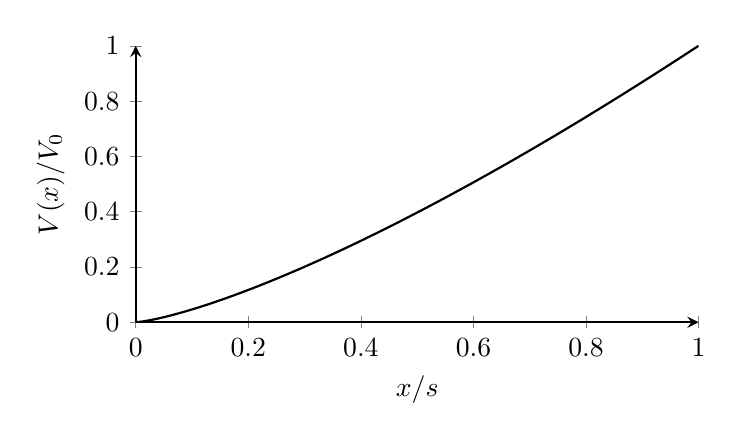
\begin{tikzpicture}
\begin{axis}[
 width=0.72\textwidth,
 height=0.42\textwidth,
 xlabel={$x/s$},
 ylabel={$V(x)/V_{0}$},
 xmin=0, xmax=1,
 ymin=0, ymax=1,
 axis lines=left,
 domain=0:1,
 samples=80,
 thick,
 black,
 every axis plot/.append style={black},
]
\addplot[black, thick] {x^(4/3)};
\end{axis}
\end{tikzpicture}
\caption{Schematic, analytically computed normalised potential profile of the collisionless Child--Langmuir space-charge sheath, $V(x)/V_{0} = (x/s)^{4/3}$, from Eq.~\eqref{eq:cl_profile_norm}. The curve is an illustrative plot of the closed-form solution, not measured or simulated data.}
\label{fig:cl_profile}
\end{figure}

\subsection{The matrix-sheath limit and sheath-width scaling}

The earlier \emph{matrix-sheath} approximation assumes ion density remains uniform at its sheath-edge value, $n_{\mathrm{i}}(x) \approx n_{0}$, throughout the layer, neglecting the acceleration-induced density fall implicit in Eq.~\eqref{eq:cl_ode}. Poisson's equation then has a constant right-hand side,
\begin{equation}
\frac{\mathrm{d}^{2}V}{\mathrm{d}x^{2}} = \frac{en_{0}}{\varepsilon_{0}},
\end{equation}
integrating, with $V(0)=0$, $V'(0)=0$, to the parabolic profile
\begin{equation}
V(x) = \frac{en_{0}}{2\varepsilon_{0}}x^{2},
\end{equation}
so the matrix-sheath width satisfying $V(s_{\mathrm{m}})=V_{0}$ is
\begin{equation}
s_{\mathrm{m}} = \sqrt{\frac{2\varepsilon_{0}V_{0}}{en_{0}}} = \lambda_{\mathrm{D}}\sqrt{\frac{2eV_{0}}{T_{\mathrm{e}}}},
\label{eq:matrix_sheath}
\end{equation}
using $\lambda_{\mathrm{D}}$ from Eq.~\eqref{appA-eq:debye}. This is the crudest self-consistent thickness estimate, exact only for an abruptly applied bias before the density relaxes to the profile implied by Eq.~\eqref{eq:cl_ode}; it remains useful for transient and pulsed-bias sheath problems \cite{ref0023}.

A more accurate estimate follows from current continuity between the Bohm flux from the presheath, $J = en_{0}u_{\mathrm{B}}$, and the space-charge-limited current of Eq.~\eqref{eq:child_langmuir}. Equating the two and solving for $s$,
\begin{equation}
s^{2} = \frac{4}{9}\frac{\varepsilon_{0}}{en_{0}}\sqrt{\frac{2e}{T_{\mathrm{e}}}}\,V_{0}^{3/2}
= \frac{4\sqrt{2}}{9}\,\lambda_{\mathrm{D}}^{2}\left(\frac{eV_{0}}{T_{\mathrm{e}}}\right)^{3/2},
\end{equation}
so that
\begin{equation}
\boxed{\frac{s}{\lambda_{\mathrm{D}}} = \left(\frac{4\sqrt{2}}{9}\right)^{1/2}\left(\frac{eV_{0}}{T_{\mathrm{e}}}\right)^{3/4} \approx 0.79\left(\frac{eV_{0}}{T_{\mathrm{e}}}\right)^{3/4}}.
\label{eq:cl_scaling}
\end{equation}
This recovers the well-known three-quarter-power scaling of collisionless sheath thickness with normalised wall bias: highly biased sheaths (large $eV_{0}/T_{\mathrm{e}}$) are many Debye lengths thick, consistent with two-fluid and kinetic sheath models \cite{ref0023}.

\subsection{Collisional correction: the mobility-limited (Mott--Gurney) sheath}

The collisionless derivation of Eq.~\eqref{eq:child_langmuir} assumes ions cross the sheath collisionlessly, which degrades as neutral pressure rises and the mean free path shortens toward $s$. In the fully collisional limit, transport is mobility-limited: $u_{\mathrm{i}}(x) = \mu E(x)$, with $\mu$ the constant ion mobility, replacing Eq.~\eqref{eq:cl_energy}. Current continuity $J = e n_{\mathrm{i}}\mu E$ and Poisson's equation $\mathrm{d}E/\mathrm{d}x = en_{\mathrm{i}}/\varepsilon_{0}$ combine to $J = \varepsilon_{0}\mu E\,\mathrm{d}E/\mathrm{d}x$. Integrating once from $E(0)=0$,
\begin{equation}
E(x) = \sqrt{\frac{2Jx}{\varepsilon_{0}\mu}},
\end{equation}
and integrating $V(x) = \int_{0}^{x} E(x')\,\mathrm{d}x'$ a second time,
\begin{equation}
V(x) = \frac{2}{3}\sqrt{\frac{2J}{\varepsilon_{0}\mu}}\,x^{3/2}.
\end{equation}
Applying $V(s) = V_{0}$ and solving for $J$ gives the Mott--Gurney law,
\begin{equation}
\boxed{J_{\mathrm{MG}} = \frac{9}{8}\,\varepsilon_{0}\mu\,\frac{V_{0}^{2}}{s^{3}}}.
\label{eq:mott_gurney}
\end{equation}
Comparing with Eq.~\eqref{eq:child_langmuir}, the collisional sheath current scales as $V_{0}^{2}$ rather than $V_{0}^{3/2}$, and $s^{-3}$ rather than $s^{-2}$ -- a signature used to identify the collisionless-to-collisional transition from measured $I$--$V$ characteristics. The resulting reduction of transmitted ion flux, and its consequences for the ion energy flux reaching the wall (Section~\ref{sec:flux}), have been analysed for elastic and charge-exchange collision channels \cite{ref0090}.

\section{Floating-Potential Expression from Flux Balance}
\label{sec:floating}

\subsection{Random thermal flux and the Bohm flux}

An electrically isolated (floating) surface draws no net current in steady state, so ion and electron fluxes at it must balance. The ion flux is fixed at the Bohm value from Section~\ref{appA-sec:bohm},
\begin{equation}
\Gamma_{\mathrm{i}} = n_{0}u_{\mathrm{B}} = n_{0}\sqrt{\frac{T_{\mathrm{e}}}{m_{\mathrm{i}}}}.
\label{eq:ion_flux_floating}
\end{equation}
The electron flux at the sheath edge, absent a retarding field, is the one-sided random thermal flux of a Maxwellian population,
\begin{equation}
\Gamma_{\mathrm{e},0} = \frac{1}{4}n_{0}\bar{v}_{\mathrm{e}},
\qquad
\bar{v}_{\mathrm{e}} = \sqrt{\frac{8T_{\mathrm{e}}}{\pi m_{\mathrm{e}}}},
\label{eq:electron_random_flux}
\end{equation}
with $\bar{v}_{\mathrm{e}}$ the mean thermal speed. Only electrons with enough normal kinetic energy overcome the retarding barrier $|V_{\mathrm{f}}|$ at a negatively floating wall; by Eq.~\eqref{appA-eq:boltzmann}, the reduction factor is $\exp(eV_{\mathrm{f}}/T_{\mathrm{e}})$, $V_{\mathrm{f}}<0$, giving
\begin{equation}
\Gamma_{\mathrm{e}}(V_{\mathrm{f}}) = \frac{1}{4}n_{0}\bar{v}_{\mathrm{e}}\exp\!\left(\frac{eV_{\mathrm{f}}}{T_{\mathrm{e}}}\right).
\label{eq:electron_wall_flux}
\end{equation}

\subsection{Flux balance and solution}

Setting $\Gamma_{\mathrm{i}} = \Gamma_{\mathrm{e}}(V_{\mathrm{f}})$ via Eqs.~\eqref{eq:ion_flux_floating}--\eqref{eq:electron_wall_flux},
\begin{equation}
n_{0}\sqrt{\frac{T_{\mathrm{e}}}{m_{\mathrm{i}}}} = \frac{1}{4}n_{0}\sqrt{\frac{8T_{\mathrm{e}}}{\pi m_{\mathrm{e}}}}\exp\!\left(\frac{eV_{\mathrm{f}}}{T_{\mathrm{e}}}\right).
\end{equation}
The factors $n_{0}$, $\sqrt{T_{\mathrm{e}}}$ cancel, leaving
\begin{equation}
\exp\!\left(\frac{eV_{\mathrm{f}}}{T_{\mathrm{e}}}\right) = \frac{4}{\sqrt{8/(\pi m_{\mathrm{e}})}}\cdot\frac{1}{\sqrt{m_{\mathrm{i}}}}
= \sqrt{\frac{16\pi m_{\mathrm{e}}}{8 m_{\mathrm{i}}}}
= \sqrt{\frac{2\pi m_{\mathrm{e}}}{m_{\mathrm{i}}}},
\end{equation}
and taking the logarithm gives the floating-potential expression
\begin{equation}
\boxed{V_{\mathrm{f}} = \frac{T_{\mathrm{e}}}{2e}\ln\!\left(\frac{2\pi m_{\mathrm{e}}}{m_{\mathrm{i}}}\right) = -\frac{T_{\mathrm{e}}}{2e}\ln\!\left(\frac{m_{\mathrm{i}}}{2\pi m_{\mathrm{e}}}\right)}.
\label{eq:floating_potential}
\end{equation}
Because $m_{\mathrm{e}} \ll m_{\mathrm{i}}$, the logarithm argument is small and $V_{\mathrm{f}}$ is negative, as required: the surface charges negatively to repel the more mobile electrons until fluxes balance. For argon, $m_{\mathrm{i}}/m_{\mathrm{e}} \approx 7.28\times10^{4}$, giving $V_{\mathrm{f}} \approx -4.68\,T_{\mathrm{e}}/e$; at $T_{\mathrm{e}} = \SI{3}{\electronvolt}$, $V_{\mathrm{f}} \approx \SI{-14.0}{\volt}$, consistent with Langmuir-probe and ion-flux diagnostics of argon discharges.

\subsection{Remarks on the flux-balance approximation}

The derivation assumes (i) a Maxwellian electron population disturbed only through the Boltzmann retardation factor, (ii) a collisionless sheath so ion flux entering equals flux striking the wall, with no volumetric ionisation or charge-exchange loss inside it, and (iii) negligible secondary electron emission. Relaxing (i) modifies both the random-flux prefactor and the retardation factor, leading to a more general sheath-formation criterion \cite{ref0090}; relaxing (ii) requires an explicit source term in the ion continuity equation, coupling to the collisional presheath models of Section~\ref{appA-sec:bohm}. Equation~\eqref{eq:floating_potential} is the reference level against which the instantaneous sheath voltage drop $\Delta\phi(t) = \phi_{\mathrm{plasma}} - \phi_{\mathrm{wall}}(t)$ is measured in Section~\ref{sec:flux}, and the natural energy origin for ion-energy distributions at floating or self-biased surfaces.

\subsection{Correction for secondary electron emission}

Ion bombardment of the wall (and, at high sheath voltage, electron bombardment) liberates secondary electrons with yield $\gamma$, the mean number emitted per incident primary. These are accelerated back across the sheath field, adding an outward current to the flux balance. Assuming every secondary escapes, the net outward electron current is augmented by $\gamma\Gamma_{\mathrm{i}}$, modifying the zero-net-current condition to
\begin{equation}
\Gamma_{\mathrm{i}} + \gamma\Gamma_{\mathrm{i}} = \Gamma_{\mathrm{e}}(V_{\mathrm{f}}'),
\qquad\text{i.e.}\qquad
(1-\gamma)^{-1}\Gamma_{\mathrm{i}} = \Gamma_{\mathrm{e}}(V_{\mathrm{f}}').
\end{equation}
Repeating the algebra of Section~\ref{sec:floating} gives the secondary-emission-corrected floating potential,
\begin{equation}
V_{\mathrm{f}}' = \frac{T_{\mathrm{e}}}{2e}\ln\!\left[\frac{2\pi m_{\mathrm{e}}}{m_{\mathrm{i}}(1-\gamma)^{2}}\right] = V_{\mathrm{f}} - \frac{T_{\mathrm{e}}}{e}\ln(1-\gamma),
\label{eq:floating_potential_see}
\end{equation}
showing secondary emission ($\gamma>0$) makes $V_{\mathrm{f}}$ \emph{less} negative than Eq.~\eqref{eq:floating_potential} predicts, since a smaller barrier now balances the augmented outward current. As $\gamma \to 1$, Eq.~\eqref{eq:floating_potential_see} diverges, signalling space-charge-limited or unstable sheath behaviour; this regime, and its diagnostic use for monitoring incident ion flux via sheath-accelerated secondary electrons, has been examined directly \cite{ref0078}.

\section{The Ion Energy Flux Integral and Its Moments}
\label{sec:flux}

\subsection{The ion velocity distribution function}

The central diagnostic quantity of this monograph is the flux of kinetic energy carried by ions across the sheath to a bounding surface, defined as a moment of the wall-normal ion velocity distribution function $f_{\mathrm{i}}(v)$, where $f_{\mathrm{i}}(v)\,\mathrm{d}v$ is the number density of ions with wall-normal velocity in $[v, v+\mathrm{d}v]$, $v \ge 0$. It is normalised so its zeroth moment recovers the local ion density,
\begin{equation}
n_{\mathrm{i}} = \int_{0}^{\infty} f_{\mathrm{i}}(v)\,\mathrm{d}v.
\label{appA-eq:moment0}
\end{equation}
The evolution of $f_{\mathrm{i}}(v)$ as ions cross the collisionless sheath, arriving broadened by presheath kinetics rather than as a mono-energetic beam, has been studied extensively \cite{ref0090,ref0672} and underlies the moment analysis below.

\subsection{Moments: particle flux, momentum flux, and energy flux}

The first velocity moment of $f_{\mathrm{i}}(v)$ gives the ion particle flux density,
\begin{equation}
\Gamma_{\mathrm{i}} = \int_{0}^{\infty} v\,f_{\mathrm{i}}(v)\,\mathrm{d}v,
\label{appA-eq:moment1}
\end{equation}
reducing to Eq.~\eqref{eq:ion_flux_floating} in the cold, mono-energetic Bohm-flux limit $f_{\mathrm{i}}(v) = n_{0}\delta(v-u_{\mathrm{B}})$. The second moment gives the ion momentum flux (dynamic pressure),
\begin{equation}
\Pi_{\mathrm{i}} = m_{\mathrm{i}}\int_{0}^{\infty} v^{2}f_{\mathrm{i}}(v)\,\mathrm{d}v,
\label{appA-eq:moment2}
\end{equation}
relevant to sputtering and erosion but not pursued further. The quantity of central interest, the \emph{ion energy flux}, is the third moment,
\begin{equation}
\boxed{\Gamma_{E} \equiv \int_{0}^{\infty} \left(\frac{1}{2}m_{\mathrm{i}}v^{2}\right)v\,f_{\mathrm{i}}(v)\,\mathrm{d}v = \frac{m_{\mathrm{i}}}{2}\int_{0}^{\infty} v^{3}f_{\mathrm{i}}(v)\,\mathrm{d}v},
\label{eq:energy_flux}
\end{equation}
with units of power per unit area: the kinetic-energy delivery rate of the ion population to the surface, the quantity ion-energy-flux sensors measure \cite{ref0075,ref0080}, setting surface heat load in plasma processing \cite{ref0080} and the power balance of fusion-relevant plasma-facing components \cite{ref0093}.

\subsection{Change of variable to energy space}

Retarding-field energy analysers resolve flux versus kinetic energy rather than velocity, motivating $v \to E = \tfrac{1}{2}m_{\mathrm{i}}v^{2}$, so $v = \sqrt{2E/m_{\mathrm{i}}}$, $\mathrm{d}v = \mathrm{d}E/\sqrt{2m_{\mathrm{i}}E}$. Defining $I_{E}(E)$ so $I_{E}(E)\,\mathrm{d}E$ is the particle flux carried by ions in $[E, E+\mathrm{d}E]$,
\begin{equation}
I_{E}(E)\,\mathrm{d}E \equiv v\,f_{\mathrm{i}}(v)\,\mathrm{d}v
\quad\Longrightarrow\quad
I_{E}(E) = \frac{v\,f_{\mathrm{i}}(v)}{m_{\mathrm{i}}v} = \frac{1}{m_{\mathrm{i}}}f_{\mathrm{i}}\!\left(\sqrt{\tfrac{2E}{m_{\mathrm{i}}}}\right).
\label{eq:iedf_def}
\end{equation}
The particle- and energy-flux moments take the compact forms
\begin{align}
\Gamma_{\mathrm{i}} &= \int_{0}^{\infty} I_{E}(E)\,\mathrm{d}E, \label{eq:gamma_i_energy} \\
\Gamma_{E} &= \int_{0}^{\infty} E\,I_{E}(E)\,\mathrm{d}E. \label{eq:gamma_E_energy}
\end{align}
$I_{E}(E)$, the flux-weighted ion energy distribution function (IEDF), is what is directly reconstructed from retarding-field-analyser or energy-selective spectrometer data \cite{ref0074,ref0090,ref0672}. The mean ion impact energy follows as
\begin{equation}
\langle E \rangle \equiv \frac{\Gamma_{E}}{\Gamma_{\mathrm{i}}} = \frac{\int_{0}^{\infty} E\,I_{E}(E)\,\mathrm{d}E}{\int_{0}^{\infty} I_{E}(E)\,\mathrm{d}E},
\label{eq:mean_energy}
\end{equation}
the single-number diagnostic most often reported alongside $\Gamma_{E}$ \cite{ref0075}.

\subsection{Sheath acceleration and the mapping from sheath-edge to wall energy}

In a collisionless sheath, an ion crossing from the sheath edge (energy $E_{0}$, of order $T_{\mathrm{e}}/2$ under Bohm-criterion equality) to the wall gains energy equal to the instantaneous potential drop traversed,
\begin{equation}
E_{\mathrm{wall}} = E_{0} + e\,\Delta\phi(t_{\mathrm{transit}}),
\label{eq:energy_gain}
\end{equation}
with $\Delta\phi(t) \equiv \phi_{\mathrm{plasma}} - \phi_{\mathrm{wall}}(t)$ the sheath voltage at the transit instant. This is the microscopic origin of the broadened, multi-peaked, or saddle-shaped IEDFs seen at rf-biased or pulsed surfaces: $I_{E}(E)$ at the wall is, to good approximation, a convolution of the sheath-edge distribution with the distribution of sheath voltages sampled during transit \cite{ref0090,ref0672}. Since Eq.~\eqref{eq:gamma_E_energy} is linear in $I_{E}(E)$, the total energy flux over a bias cycle is the transit-weighted average of the instantaneous flux, exploited by the reconstruction procedures of Sections~\ref{sec:tikhonov}--\ref{sec:bayes}. This connects to non-Maxwellian sheath-formation criteria \cite{ref0090}, the flux distribution's tail behaviour \cite{ref0096}, and global energy accounting of ion bombardment on plasma-facing surfaces \cite{ref0093}.

\subsection{Higher moments: energy spread and the flux-weighted variance}

The mean impact energy of Eq.~\eqref{eq:mean_energy} does not characterise distribution width, which matters for diagnostic energy resolution and threshold sputtering. The flux-weighted energy variance is defined via the raw second moment,
\begin{equation}
\langle E^{2}\rangle \equiv \frac{1}{\Gamma_{\mathrm{i}}}\int_{0}^{\infty} E^{2}\,I_{E}(E)\,\mathrm{d}E,
\qquad
\operatorname{Var}[E] = \langle E^{2}\rangle - \langle E\rangle^{2}.
\label{eq:energy_variance}
\end{equation}
For a narrow, quasi-mono-energetic population from a low-voltage collisionless sheath, $\operatorname{Var}[E] \to 0$; a time-modulated sheath voltage, an rf-biased surface, or a collisional presheath instead increases $\operatorname{Var}[E]$, via the linear mapping of Eq.~\eqref{eq:energy_gain}. Since Eqs.~\eqref{eq:gamma_i_energy}, \eqref{eq:gamma_E_energy}, and~\eqref{eq:energy_variance} are all linear functionals of $I_{E}(E)$, they can be evaluated directly, with propagated uncertainty, from the reconstruction of $I_{E}(E)$ in Sections~\ref{sec:tikhonov}--\ref{sec:bayes}. Whether $I_{E}(E)$ decays algebraically or exponentially at large $E$ determines the stability of these moment integrals, addressed by dedicated studies of the predicted PDF tails of the sheath ion flux \cite{ref0096}.

\section{Tikhonov-Regularised Least-Squares Solution}
\label{sec:tikhonov}

\subsection{The linear inverse problem}

The quantities of Section~\ref{sec:flux} -- chiefly $I_{E}(E)$, discretised as $\mathbf{m} \in \mathbb{R}^{N}$ on a chosen energy grid -- are not measured directly. A diagnostic instrument instead records $\mathbf{d} \in \mathbb{R}^{M}$ related to $\mathbf{m}$ through a known linear forward operator $\mathbf{K} \in \mathbb{R}^{M\times N}$ (the instrument response kernel) contaminated by additive noise $\mathbf{n}$,
\begin{equation}
\mathbf{d} = \mathbf{K}\mathbf{m} + \mathbf{n}.
\label{eq:forward_model}
\end{equation}
This is the canonical linear inverse problem in plasma spectroscopic and flux diagnostics \cite{ref0677,ref0687}, generically ill-posed in Hadamard's sense: $\mathbf{K}$ is typically ill-conditioned, so naive least-squares inversion amplifies noise without bound.

\subsection{Ordinary least squares and its failure}

The unregularised least-squares estimate minimises the residual sum of squares,
\begin{equation}
\hat{\mathbf{m}}_{\mathrm{OLS}} = \arg\min_{\mathbf{m}} \|\mathbf{K}\mathbf{m} - \mathbf{d}\|_{2}^{2},
\end{equation}
with formal solution $\hat{\mathbf{m}}_{\mathrm{OLS}} = (\mathbf{K}^{\mathsf{T}}\mathbf{K})^{-1}\mathbf{K}^{\mathsf{T}}\mathbf{d}$ whenever $\mathbf{K}^{\mathsf{T}}\mathbf{K}$ is invertible. With the SVD $\mathbf{K} = \mathbf{U}\boldsymbol{\Sigma}\mathbf{V}^{\mathsf{T}}$, singular values $\sigma_{i}$, $\hat{\mathbf{m}}_{\mathrm{OLS}} = \sum_{i} \sigma_{i}^{-1}(\mathbf{u}_{i}^{\mathsf{T}}\mathbf{d})\mathbf{v}_{i}$: components with small $\sigma_{i}$ are amplified catastrophically, rendering $\hat{\mathbf{m}}_{\mathrm{OLS}}$ noise-dominated whenever $\mathbf{K}$ is ill-conditioned, generically true for energy-resolving sheath diagnostics \cite{ref0695}.

\subsection{Tikhonov regularisation and the normal equations}

Tikhonov regularisation stabilises the inversion by augmenting the least-squares objective with a penalty on the size (or roughness) of the solution, via a regularisation operator $\mathbf{L}$ (identity for zeroth-order regularisation, or a discrete derivative operator to enforce smoothness):
\begin{equation}
J(\mathbf{m}) = \|\mathbf{K}\mathbf{m} - \mathbf{d}\|_{2}^{2} + \alpha^{2}\|\mathbf{L}\mathbf{m}\|_{2}^{2},
\label{eq:tikhonov_functional}
\end{equation}
with $\alpha > 0$ controlling the data-fidelity/smoothness trade-off. Expanding,
\begin{equation}
J(\mathbf{m}) = \mathbf{m}^{\mathsf{T}}\mathbf{K}^{\mathsf{T}}\mathbf{K}\mathbf{m} - 2\mathbf{d}^{\mathsf{T}}\mathbf{K}\mathbf{m} + \mathbf{d}^{\mathsf{T}}\mathbf{d} + \alpha^{2}\mathbf{m}^{\mathsf{T}}\mathbf{L}^{\mathsf{T}}\mathbf{L}\mathbf{m},
\end{equation}
and differentiating, the stationarity condition is
\begin{equation}
\nabla_{\mathbf{m}} J = 2\mathbf{K}^{\mathsf{T}}(\mathbf{K}\mathbf{m} - \mathbf{d}) + 2\alpha^{2}\mathbf{L}^{\mathsf{T}}\mathbf{L}\mathbf{m} = \mathbf{0},
\end{equation}
which rearranges to the Tikhonov \emph{normal equations},
\begin{equation}
\boxed{\left(\mathbf{K}^{\mathsf{T}}\mathbf{K} + \alpha^{2}\mathbf{L}^{\mathsf{T}}\mathbf{L}\right)\mathbf{m}_{\alpha} = \mathbf{K}^{\mathsf{T}}\mathbf{d}},
\label{eq:normal_equations}
\end{equation}
with unique solution
\begin{equation}
\mathbf{m}_{\alpha} = \left(\mathbf{K}^{\mathsf{T}}\mathbf{K} + \alpha^{2}\mathbf{L}^{\mathsf{T}}\mathbf{L}\right)^{-1}\mathbf{K}^{\mathsf{T}}\mathbf{d}
\label{eq:tikhonov_solution}
\end{equation}
for $\alpha>0$, since $\mathbf{K}^{\mathsf{T}}\mathbf{K} + \alpha^{2}\mathbf{L}^{\mathsf{T}}\mathbf{L}$ is then strictly positive definite even when $\mathbf{K}^{\mathsf{T}}\mathbf{K}$ alone is singular. This, or its numerically preferable augmented-system equivalent, underlies most applied inversion methods for spectroscopic and flux-diagnostic reconstruction in plasma physics \cite{ref0677}.

\subsection{Filter-factor interpretation and choice of $\alpha$}

For $\mathbf{L} = \mathbf{I}$, substituting the SVD into Eq.~\eqref{eq:tikhonov_solution} gives the filter-factor form
\begin{equation}
\mathbf{m}_{\alpha} = \sum_{i} \frac{\sigma_{i}^{2}}{\sigma_{i}^{2}+\alpha^{2}}\cdot\frac{\mathbf{u}_{i}^{\mathsf{T}}\mathbf{d}}{\sigma_{i}}\,\mathbf{v}_{i},
\label{eq:filter_factors}
\end{equation}
showing regularisation damps components with $\sigma_{i} \ll \alpha$ (filter factor $\to 0$) while leaving well-determined components with $\sigma_{i} \gg \alpha$ essentially undamped ($\to 1$). Too small an $\alpha$ reproduces the noise amplification of ordinary least squares; too large over-smooths, biasing moments such as $\Gamma_{E}$ and $\langle E\rangle$. Practical selection strategies -- the discrepancy principle, generalised cross-validation, and the L-curve criterion (the corner of maximum curvature of $\log\|\mathbf{K}\mathbf{m}_{\alpha}-\mathbf{d}\|$ versus $\log\|\mathbf{L}\mathbf{m}_{\alpha}\|$) -- are discussed in the regularisation literature applied to spectroscopic and tomographic plasma inversions \cite{ref0677,ref0695}.

\subsection{Generalised (weighted) Tikhonov regularisation}

When measurement noise is heteroscedastic and correlated, described by a data covariance $\boldsymbol{\Sigma}_{d}$, and prior information is encoded through a prior covariance $\boldsymbol{\Sigma}_{m}$ about a reference model $\mathbf{m}_{0}$, the natural generalisation of Eq.~\eqref{eq:tikhonov_functional} is the weighted objective
\begin{equation}
J(\mathbf{m}) = (\mathbf{K}\mathbf{m}-\mathbf{d})^{\mathsf{T}}\boldsymbol{\Sigma}_{d}^{-1}(\mathbf{K}\mathbf{m}-\mathbf{d}) + (\mathbf{m}-\mathbf{m}_{0})^{\mathsf{T}}\boldsymbol{\Sigma}_{m}^{-1}(\mathbf{m}-\mathbf{m}_{0}),
\label{eq:generalised_tikhonov}
\end{equation}
reducing to Eq.~\eqref{eq:tikhonov_functional} for $\boldsymbol{\Sigma}_{d} = \sigma_{d}^{2}\mathbf{I}$, $\mathbf{m}_{0}=\mathbf{0}$, $\boldsymbol{\Sigma}_{m}^{-1} = (\alpha^{2}/\sigma_{d}^{2})\mathbf{L}^{\mathsf{T}}\mathbf{L}$, and forming the direct bridge to the Bayesian formulation developed next, where $\boldsymbol{\Sigma}_{d}$ and $\boldsymbol{\Sigma}_{m}$ acquire an explicit probabilistic interpretation \cite{ref0683,ref0684,ref0685,ref0687}.

\subsection{Numerical solution of the normal equations}

Forming and inverting $\mathbf{K}^{\mathsf{T}}\mathbf{K}$ explicitly is undesirable: its condition number is the square of that of $\mathbf{K}$. Two strategies are preferred. Since $\mathbf{K}^{\mathsf{T}}\mathbf{K}+\alpha^{2}\mathbf{L}^{\mathsf{T}}\mathbf{L}$ is symmetric positive definite for $\alpha>0$, Eq.~\eqref{eq:normal_equations} may be solved by Cholesky factorisation, $\mathbf{K}^{\mathsf{T}}\mathbf{K}+\alpha^{2}\mathbf{L}^{\mathsf{T}}\mathbf{L} = \mathbf{R}^{\mathsf{T}}\mathbf{R}$, followed by two triangular back-substitutions. More robust for strongly ill-conditioned $\mathbf{K}$ is the equivalent augmented least-squares problem,
\begin{equation}
\mathbf{m}_{\alpha} = \arg\min_{\mathbf{m}} \left\|
\begin{pmatrix}\mathbf{K}\\ \alpha\mathbf{L}\end{pmatrix}\mathbf{m}
-
\begin{pmatrix}\mathbf{d}\\ \mathbf{0}\end{pmatrix}
\right\|_{2}^{2},
\label{eq:augmented_ls}
\end{equation}
solved by $QR$ or SVD factorisation of the stacked matrix without ever forming $\mathbf{K}^{\mathsf{T}}\mathbf{K}$. Exploring the bias--variance trade-off across trial $\alpha$ is then dominated by a single factorisation of $\mathbf{K}$, after which solution and residual norms follow from Eq.~\eqref{eq:filter_factors} at negligible cost \cite{ref0677}.

\section{Bayesian MAP Estimate for a Gaussian Prior and Likelihood}
\label{sec:bayes}

\subsection{Likelihood and prior}

The Bayesian formulation treats the unknown model $\mathbf{m}$ as a random vector, updated in light of the data $\mathbf{d}$ via Bayes' theorem. With additive Gaussian noise of covariance $\boldsymbol{\Sigma}_{d}$, the likelihood is
\begin{equation}
p(\mathbf{d}\mid\mathbf{m}) \propto \exp\!\left[-\tfrac{1}{2}(\mathbf{d}-\mathbf{K}\mathbf{m})^{\mathsf{T}}\boldsymbol{\Sigma}_{d}^{-1}(\mathbf{d}-\mathbf{K}\mathbf{m})\right].
\label{appA-eq:likelihood}
\end{equation}
A Gaussian prior, reflecting expected smoothness or agreement with a fluid-theory prediction $\mathbf{m}_{0}$ from Sections~\ref{appA-sec:bohm}--\ref{sec:flux}, is written
\begin{equation}
p(\mathbf{m}) \propto \exp\!\left[-\tfrac{1}{2}(\mathbf{m}-\mathbf{m}_{0})^{\mathsf{T}}\boldsymbol{\Sigma}_{m}^{-1}(\mathbf{m}-\mathbf{m}_{0})\right].
\label{eq:prior}
\end{equation}
This Gaussian-linear setting is the standard starting point for Bayesian analysis of plasma diagnostics \cite{ref0683,ref0684,ref0685} and for inverse problems more broadly \cite{ref0687}.

\subsection{The posterior and the MAP estimate}

By Bayes' theorem, the posterior is proportional to the product of likelihood and prior,
\begin{equation}
p(\mathbf{m}\mid\mathbf{d}) \propto p(\mathbf{d}\mid\mathbf{m})\,p(\mathbf{m}),
\end{equation}
and, both factors Gaussian in $\mathbf{m}$, so is the posterior. The MAP estimate maximises $p(\mathbf{m}\mid\mathbf{d})$, equivalently minimising the negative log-posterior,
\begin{equation}
J_{\mathrm{MAP}}(\mathbf{m}) = (\mathbf{d}-\mathbf{K}\mathbf{m})^{\mathsf{T}}\boldsymbol{\Sigma}_{d}^{-1}(\mathbf{d}-\mathbf{K}\mathbf{m}) + (\mathbf{m}-\mathbf{m}_{0})^{\mathsf{T}}\boldsymbol{\Sigma}_{m}^{-1}(\mathbf{m}-\mathbf{m}_{0}),
\label{eq:map_functional}
\end{equation}
identical in form to the generalised Tikhonov functional of Eq.~\eqref{eq:generalised_tikhonov}. Differentiating and setting the gradient to zero,
\begin{equation}
-2\mathbf{K}^{\mathsf{T}}\boldsymbol{\Sigma}_{d}^{-1}(\mathbf{d}-\mathbf{K}\mathbf{m}) + 2\boldsymbol{\Sigma}_{m}^{-1}(\mathbf{m}-\mathbf{m}_{0}) = \mathbf{0},
\end{equation}
rearranges, exactly as in Section~\ref{sec:tikhonov}, to the MAP normal equations
\begin{equation}
\left(\mathbf{K}^{\mathsf{T}}\boldsymbol{\Sigma}_{d}^{-1}\mathbf{K} + \boldsymbol{\Sigma}_{m}^{-1}\right)\mathbf{m}_{\mathrm{MAP}} = \mathbf{K}^{\mathsf{T}}\boldsymbol{\Sigma}_{d}^{-1}\mathbf{d} + \boldsymbol{\Sigma}_{m}^{-1}\mathbf{m}_{0},
\end{equation}
with explicit solution
\begin{equation}
\boxed{\mathbf{m}_{\mathrm{MAP}} = \left(\mathbf{K}^{\mathsf{T}}\boldsymbol{\Sigma}_{d}^{-1}\mathbf{K} + \boldsymbol{\Sigma}_{m}^{-1}\right)^{-1}\left(\mathbf{K}^{\mathsf{T}}\boldsymbol{\Sigma}_{d}^{-1}\mathbf{d} + \boldsymbol{\Sigma}_{m}^{-1}\mathbf{m}_{0}\right)}.
\label{eq:map_solution}
\end{equation}

\subsection{Equivalence with Tikhonov regularisation and the regularisation parameter}

Comparing Eq.~\eqref{eq:map_solution} with the generalised Tikhonov solution shows the two estimators coincide term by term: the Bayesian MAP estimate under Gaussian likelihood and prior is \emph{identical} to the generalised Tikhonov estimate, with $\boldsymbol{\Sigma}_{d}^{-1}$ as data-weighting matrix and $\boldsymbol{\Sigma}_{m}^{-1}$ as regularisation operator. In the isotropic case $\boldsymbol{\Sigma}_{d} = \sigma_{d}^{2}\mathbf{I}$, $\boldsymbol{\Sigma}_{m}^{-1} = (\alpha^{2}/\sigma_{d}^{2})\mathbf{L}^{\mathsf{T}}\mathbf{L}$, this gives $\alpha$ explicit physical meaning: the ratio of assumed measurement-noise variance to prior-model variance,
\begin{equation}
\alpha^{2} = \sigma_{d}^{2}\left[\boldsymbol{\Sigma}_{m}\right]^{-1}_{\text{scale}},
\end{equation}
so regularisation-parameter selection can equivalently be framed as choosing plausible noise and prior variances, exploited in Bayesian plasma-diagnostic inversion frameworks \cite{ref0683,ref0684,ref0685} and the general inverse-problems literature \cite{ref0687}.

\subsection{Posterior covariance and uncertainty quantification}

Beyond a point estimate, the Gaussian-linear structure yields the full posterior covariance in closed form,
\begin{equation}
\boldsymbol{\Sigma}_{\mathrm{post}} = \left(\mathbf{K}^{\mathsf{T}}\boldsymbol{\Sigma}_{d}^{-1}\mathbf{K} + \boldsymbol{\Sigma}_{m}^{-1}\right)^{-1},
\label{eq:posterior_covariance}
\end{equation}
exactly the matrix inverted in Eq.~\eqref{eq:map_solution}. This propagates directly into uncertainty bounds on any linear functional of the reconstructed model, in particular the ion energy flux and its moments of Section~\ref{sec:flux}: for $g(\mathbf{m}) = \mathbf{c}^{\mathsf{T}}\mathbf{m}$ (e.g.\ a discretised $\Gamma_{E}$ or $\langle E\rangle$), the posterior variance is $\mathrm{Var}[g] = \mathbf{c}^{\mathsf{T}}\boldsymbol{\Sigma}_{\mathrm{post}}\mathbf{c}$, giving a formal, propagated credible interval rather than a bare point estimate. This capacity for principled uncertainty quantification is the central practical advantage of the Bayesian MAP framework over a bare Tikhonov point estimate, exploited in Bayesian reconstructions of plasma parameters from indirect spectroscopic and scattering measurements \cite{ref0683,ref0684,ref0685}, and in the wider family of regularised-inversion techniques for magnetohydrodynamic and other plasma inverse problems \cite{ref0687}.

\subsection{Hyperparameter estimation and hierarchical extensions}

The MAP formulation presupposes $\boldsymbol{\Sigma}_{d}$ and $\boldsymbol{\Sigma}_{m}$ (or, isotropically, $\sigma_{d}^{2}$, $\alpha^{2}$) are known in advance. In practice they are estimated by maximising the \emph{marginal likelihood}, or Bayesian evidence, obtained by integrating the joint density of Eqs.~\eqref{appA-eq:likelihood}--\eqref{eq:prior} over $\mathbf{m}$,
\begin{equation}
p(\mathbf{d}\mid\sigma_{d}^{2},\alpha^{2}) = \int p(\mathbf{d}\mid\mathbf{m},\sigma_{d}^{2})\,p(\mathbf{m}\mid\alpha^{2})\,\mathrm{d}\mathbf{m}.
\label{eq:evidence}
\end{equation}
Both factors being Gaussian in $\mathbf{m}$, the integral is closed-form, yielding a marginal likelihood Gaussian in $\mathbf{d}$ with covariance $\mathbf{K}\boldsymbol{\Sigma}_{m}\mathbf{K}^{\mathsf{T}} + \boldsymbol{\Sigma}_{d}$; maximising over $\sigma_{d}^{2}$, $\alpha^{2}$ gives a data-driven alternative to the L-curve and discrepancy-principle heuristics of Section~\ref{sec:tikhonov}, generalising to a hierarchical treatment where $\sigma_{d}^{2}$, $\alpha^{2}$ are assigned weak (e.g.\ inverse-gamma) hyperpriors rather than fixed at evidence-maximising values. This evidence-based approach is standard in Bayesian analyses of indirect plasma diagnostics, including multi-instrument and Gaussian-process reconstructions of scattering and interferometric data \cite{ref0683,ref0685}, and gives an objective, reproducible route to choosing $\alpha$ when reconstructing the ion energy flux distribution of Section~\ref{sec:flux} from a finite, noisy set of diagnostic channels.

\subsection{Summary}

This appendix forms a single chain from the microscopic electrostatics of a quasi-neutral plasma to the statistical machinery used elsewhere in this monograph to reconstruct a diagnostic quantity from noisy data. Linearised Poisson--Boltzmann theory (Section~\ref{appA-sec:debye}) establishes the Debye length $\lambda_{\mathrm{D}}$, the screening scale separating the quasi-neutral bulk from the non-neutral sheath. Expansion of the cold-fluid sheath equation (Section~\ref{appA-sec:bohm}) yields the Bohm criterion, $u_{0}\ge u_{\mathrm{B}}$, with its kinetic generalisation as an integral inequality. Solving the electron-free, high-voltage sheath equation (Section~\ref{sec:cl}) produces the Child--Langmuir space-charge law and its matrix-sheath and three-quarter-power scaling limits. A kinetic flux-balance argument (Section~\ref{sec:floating}) yields the floating-potential expression anchoring the energy origin of ion-impact-energy measurements. The ion energy flux is then defined as the third velocity moment of the ion distribution function (Section~\ref{sec:flux}), its zeroth and first moments recovering ion density and particle flux, and its ratio $\Gamma_{E}/\Gamma_{\mathrm{i}}$ defining the mean impact energy. Finally, Sections~\ref{sec:tikhonov} and~\ref{sec:bayes} develop the Tikhonov-regularised least-squares estimator and its exact Bayesian MAP equivalent for reconstructing the ion energy flux from noisy, indirect diagnostic measurements, culminating in a closed-form posterior covariance that supplies rigorous, propagated uncertainty bounds on the reconstructed energy flux.
